\documentclass[paper=a4, fontsize=11pt, UTF8]{article} % A4 paper and 11pt font size
\usepackage[a4paper,left=3cm,right=3cm,top=2.5cm,bottom=2.5cm]{geometry}
\usepackage{ctex}
%\usepackage[T1]{fontenc} % Use 8-bit encoding that has 256 glyphs
%\usepackage{fourier} % Use the Adobe Utopia font for the document - comment this line to return to the LaTeX default
\usepackage[english]{babel} % English language/hyphenation
\usepackage{amsmath,amsfonts,amsthm} % Math packages
\usepackage{graphicx}
\usepackage{listings}
\usepackage{xcolor}
\usepackage{siunitx}
\usepackage{booktabs}
\usepackage{multirow}
\usepackage{longtable}
\usepackage{hyperref}
\usepackage{float}
\hypersetup{
    colorlinks,
    citecolor=black,
    filecolor=black,
    linkcolor=black,
    urlcolor=black
}

\definecolor{vgreen}{RGB}{104,180,104}
\definecolor{vblue}{RGB}{49,49,255}
\definecolor{vorange}{RGB}{255,143,102}
\lstset
{
    backgroundcolor=\color[RGB]{245,245,244},
    basicstyle={\footnotesize\ttfamily},        % set code style
    keywordstyle=\color{vblue},
    identifierstyle=\color{black},
    commentstyle=\color{vgreen},
    % numbers=left,                      % set line numbers
    numberstyle={\tiny \color{black}}, % set fonts of line numbers
    frame=lines,                      % set type of open 
    numbersep=10pt,
    breaklines=true,                   % automatic line break
    tabsize=4,
    aboveskip=10pt,
    belowskip=2pt
}


\title{\fontsize{18}\baselineskip 4over6实验报告}

\author{李文凯\quad 2016011369 \quad 计65\\王 \; 琛 \quad 2016011360 \quad 计65}
\date{\normalsize\today} % Today's date or a custom date

\begin{document}

\maketitle % Print the title

\fontsize{11pt}{18pt}\selectfont
%\newpage

\section{实验目的}

\begin{itemize}
\item 掌握Android下应用程序开发环境的搭建和使用
\item 掌握IPv4 over IPv6隧道的工作原理
\end{itemize}


\section{实验原理}
4over6隧道模式是指,将ipv4报文作为载荷填入ipv6报文中,Android终端发出的报文由过渡网关负责解封并将ipv4报文发送到公网,同时过渡网关将受到的ipv4网络数据加以封装,发给Android终端。
\begin{figure}[H]
    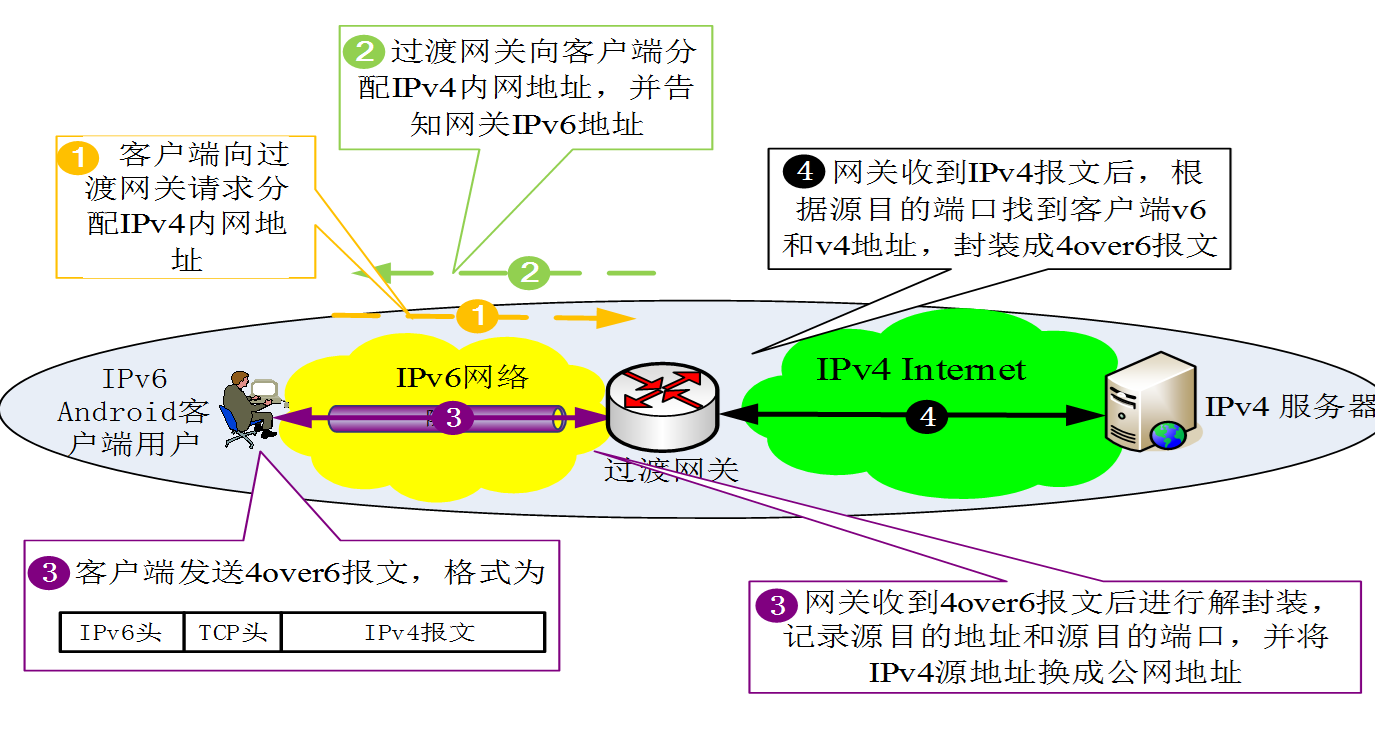
\includegraphics[width=\textwidth]{photos/fig1.png}
\end{figure}
从图中可以看出,安卓客户端首先向过渡网关分配IPv4内网地址,然后过渡网关再提供IPv4地址。然后,安卓客户端发送4over6协议报文,过渡网关接受报文并进行分析,得到源地址和目的地址,将IPv4地址转化为公网地址,发送到公网中。当过渡网关收到公网的IPv4报文之后,根据记录好的映射关系,重新封装成4over6报文,发给对应的客户端,从而完成数据的转发和接受。

在以上流程中,用户处于纯IPv6网络环境之中,过渡网关运行双栈协议。


\section{实验设计与内容}
\subsection{实验分工}
本次实验李文凯同学负责客户端,王琛同学负责客户端的流量显示部分以及服务器端。

\subsection{客户端}

\subsubsection{功能划分}
客户端程序主要分成两个模块,前台由Android编写,主要是接受用户的输入和相关指令,启用VPNService,并显示流量统计信息,而后端由C++编写,负责网络数据收发。二者调用基于JNI实现,数据交互通过管道实现。

\subsubsection{主要技术}
\paragraph{JNI与NDK}
对于网络相关的操作,往往在字节层面,并且对于内存管理的要求也更高,使用Java不便,因此还是采用了惯用的C/C++进行网络数据交互处理,由此需要在基于Java的Android开发工作中引入C/C++模块,所以我们需要使用JNI和NDK。

​JNI(Java Native Interface)提供了若干的API实现了Java和其他语言的通信,使得我们在本实验中能够实现本地方法native method,并在Java程序中调用他们。而NDK(Native Development Kit)则是方便开发者将C/C++程序打包并加入到APK中,供Android程序使用。

​当前最新的Android Studio已经提供了完善的JNI支持,相比之前,省去了编译头文件等复杂操作,框架部分已经由内置模板实现,十分方便。

\paragraph{VPNService}
\begin{itemize}
    \item 应用程序使用socket,将相应的数据包发送到真实的网络设备上。一般移动设备只有无线网卡,因此是发送到真实的WiFi设备上;
    \item Android系统通过iptables,使用NAT,将所有的数据包转发到TUN虚拟网络设备上去,端口是tun0;
    \item VPN程序通过打开/dev/tun设备,并读取该设备上的数据,可以获得所有转发到TUN虚拟网络设备上的IP包。因为设备上的所有IP包都会被NAT转成原地址是tun0端口发送的,所以也就是说你的VPN程序可以获得进出该设备的几乎所有的数据(也有例外,不是全部,比如回环数据就无法获得);
    \item VPN数据可以做一些处理,然后将处理过后的数据包,通过真实的网络设备发送出去。为了防止发送的数据包再被转到TUN虚拟网络设备上,VPN程序所使用的socket必须先被明确绑定到真实的网络设备上去。
\end{itemize}
在实际使用中,需要将Android设备与过渡网关相联的v6 socket保护起来,其他连接则纳入VPNService管辖范围。

\paragraph{管道}
管道其实就是特殊的文件,不同语言下数据交互可以就可以通过文件读写操作来完成。有两个地方需要注意:
\begin{itemize}
    \item 管道是持久化存储在设备外存的,如果程序退出未进行清理,下次运行程序仍会读取到上次的残留信息,可能引发错误。
    \item 双向读写or单向读写?本次实验为了简化操作逻辑,每个管道都是一方可读另一方可写,否则需要额外的判断或同步机制。
\end{itemize}

\subsubsection{整体工作流程}
\begin{figure}[H]
    \centering
    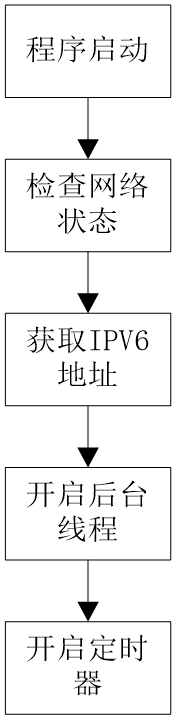
\includegraphics[scale=0.7]{photos/total.png}
\end{figure}

\subsubsection{前台}
\begin{figure}[H]
    \centering
    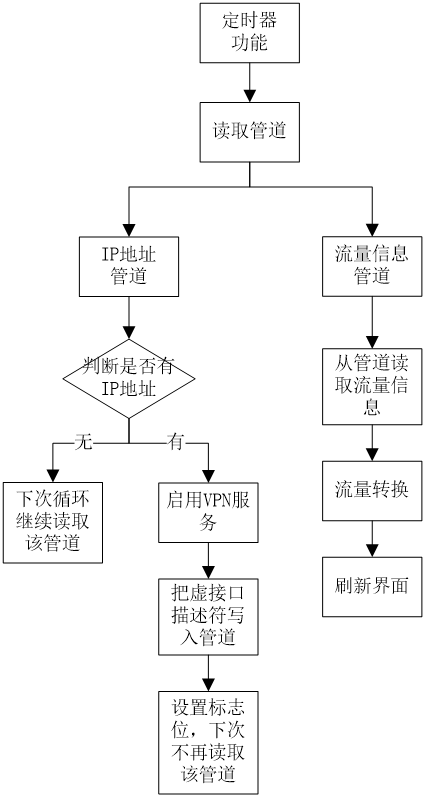
\includegraphics[scale=0.7]{photos/front.png}
\end{figure}
前台的工作总结为以下几个:
\begin{itemize}
    \item 读取用户输入的过渡网关ipv6\_address, port,传给后台线程用来发出连接请求
    \item 接受后台获得的来自过渡网关的连接响应,用来启用VPNService,并将生成的tun0描述符传给后台,供其进行数据交互
    \item 定时获取来自后台的流量统计信息,并显示。
\end{itemize}

实现要点:
\begin{itemize}
    \item backend后台线程:在点击连接按钮后,创建线程运行native method执行后台线程
    \item 定时服务:由Java提供的TimerTask实现
    \item VPNService:继承Android提供的VpnService实现
\end{itemize}

\subsubsection{后台}
后台工作流程如图所示
\begin{figure}[H]
    \centering
    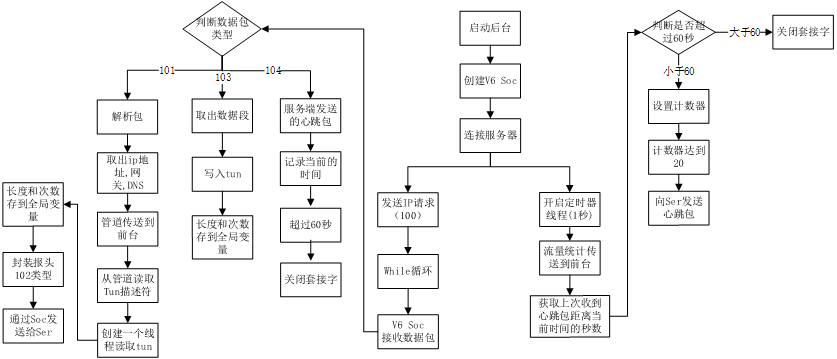
\includegraphics[scale=0.5]{photos/back.png}
\end{figure}
后台主要有以下几个重要的工作线程:
\begin{itemize}
    \item 读取ip\_pipe:获取VPNService创建的虚接口,以及程序退出信号
    \item 读取虚接口tun0:Android设备所有的上网请求都会发送到tun0,该线程负责对其进行封装,发送到过渡网关
    \item 读取ipv6 socket:获取来自过渡网关的数据,分类别进行处理
    \item 计时器:保活机制,发送流量统计信息到前台
\end{itemize}

实现要点:

后台主要是C/C++的处理逻辑,除了基础的多线程处理之外没有其他需要额外注意的地方。但是在现有的实现框架下,多个线程对一个socket进行读写操作,经过调研,Linux下的send函数并不是原子操作,因此可能出现发送心跳包的同时,发送上网请求包,导致混包的情况出现,因此必须给socket的读写操作加锁,防止该情形的发生。

\subsection{服务器}
\subsubsection{工作流程}
服务器的总体工作流程如图:
\begin{figure}[H]
    \centering
    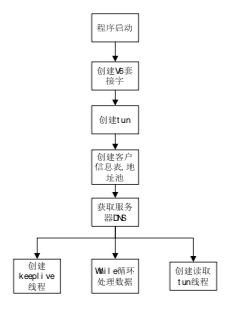
\includegraphics[scale=0.7]{photos/server.png}
\end{figure}
主要分为如下三个部分:
\begin{enumerate}
    \item 主进程接受客户端连接,接受不同类型的数据包。
    \item 创建keepalive线程,给每个正在连接的客户端发送心跳包。
    \item 读取虚接口,包括将数据发送出去,以及接受虚接口数据然后发送给客户端。
\end{enumerate}

\subsubsection{具体实现}
具体的客户端实现我们采用了近年来比较流行的epoll模型,用来代替实验指导书的select模型。使用epoll模型能够进行I/O多路复用,只用单线程即可完成任务(keepalive仍然需要新的线程)。并且epoll模型不像select模型有最大用户数目的限制,因此有了广泛的使用。

使用epoll,遍历所有的事件,可以方便判断是新的用户请求连接,还是接收到了用户数据,或者接收到了虚接口tun的数据,再做相应的处理。监听所有客户端的socket,当其中一个socket可以读或者可以写时,首先找到socket对应的用户,然后根据类型做处理。如果socket可写,则从该用户对应的数据队列中取出数据然后写入socket。如果socket可读,则读取消息,然后写到tun。tun同样注册入epoll。如果tun接收到了数据,那么进行将其转发给客户端。代码框架如下,省略了一些细节的处理。
\begin{lstlisting}[language=c++]
    while(true) {
        nfds = epoll_wait(epfd, events, 20, 500);
        for(int i = 0; i < nfds; i++) {
            if(events[i].data.fd == listenfd) { //listen event
                printf("listening event\n");
                connfd = accept(listenfd, (struct sockaddr *)&clientaddr, &client_len);
                client_fd = connfd;
                if (connfd == -1) {
                    perror("accept failed");
                    close(connfd);
                    exit(-1);
                }
                printf("client fd: %d\n", client_fd);

                int i = 0;
                pthread_mutex_lock(&mutex);
                for (; i < MAX_USER; i++) {
                    if (user_info_table[i].fd == -1) {
                        user_info_table[i].fd = connfd;
                        memcpy(&(user_info_table[i].v6addr), &clientaddr, sizeof(struct sockaddr));
                        user_info_table[i].secs = time(NULL);
                        user_info_table[i].count = 5;
                        break;
                    }
                }
                pthread_mutex_unlock(&mutex);

                //accept connection
            } else { 
                if(events[i].data.fd == tun_fd) {
                    process_packet_to_tun(client_fd);
                } else if(events[i].events & EPOLLIN) {
                    //receive from user
                }
            }
        }
    }
\end{lstlisting}
开始运行时,首先要打开服务器的监听socket,具体实现的IPv4的情况十分类似,只是需要将其修改为IPv6情形下。设置完监听之后,将其放入epoll中。
\begin{lstlisting}[language=c++]
    struct sockaddr_in6 server_addr;
    server_addr.sin6_family = AF_INET6;
    server_addr.sin6_addr = in6addr_any;
    server_addr.sin6_port = htons(SERVER_PORT);
    int ret = bind(listenfd, (struct sockaddr *) &server_addr, sizeof(server_addr));
    if (ret == -1) {
        perror("server bind error");
        close(listenfd);
        exit(-1);
    }
    if( (ret=listen(listenfd, MAX_USER)) < 0 ) {
        perror("Server listen failed");
    }
\end{lstlisting}

用户信息根据实验指导书,保存在user\_info的结构体中。每个用户分配一个ip地址和一个socket。使用keepalive线程,每隔一秒钟向用户放松心跳包,当某个用户发送的心跳包超时时,则从队列中删除掉该用户。注意keepalive线程发送包时需要加上锁,防止写数据出错。

在服务器端,使用iptables做NAT,实现私有网段和公网地址的转换。在c++中可以使用system函数运行shell命令。iptables会建立和服务器端口之间的映射,并且将IP报文的源地址、源端口转换为服务器的公网IP和端口。我们使用10.0.0.1/24作为私有网段。相关的一些配置如下:
\begin{lstlisting}[language=c++]
    char buffer[256];
    sprintf(buffer,"ip link set dev %s up", ifr.ifr_name);
    system(buffer);
    sprintf(buffer,"ip a add 10.0.0.1/24 dev %s", ifr.ifr_name);
    system(buffer);
    sprintf(buffer,"ip link set dev %s mtu %u", ifr.ifr_name, 1500 - MSG_HEADER_SIZE);
    system(buffer);
\end{lstlisting}

\subsubsection{编译运行}
server文件夹下已经有makefile,使用make命令即可编译,开启了pthread和std=c++11的编译选项

使用make run命令可以运行

\subsubsection{运行情况}
下图是服务器收到用户包和发送包给用户的情况:
\begin{figure}[H]
	\centering %图片全局居中
	%并排几个图,就要写几个minipage
	\begin{minipage}[b]{0.45\textwidth} %所有minipage宽度之和要小于1,否则会自动变成竖排
		\centering %图片局部居中
		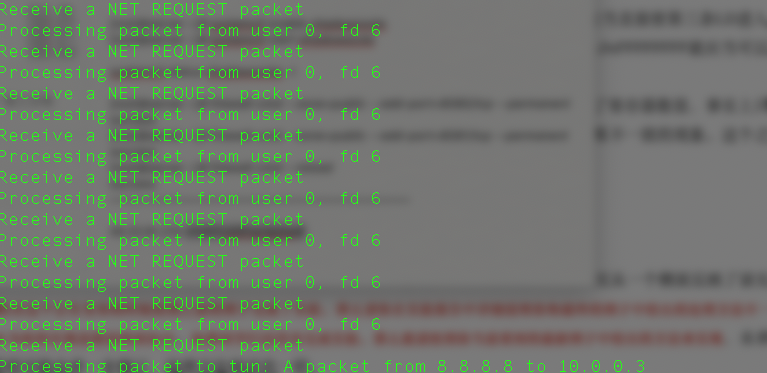
\includegraphics[scale=0.25]{./photos/1.png} %此时的图片宽度比例是相对于这个minipage的,不是全局
	\end{minipage}
	\begin{minipage}[b]{0.45\textwidth} %所有minipage宽度之和要小于1,否则会自动变成竖排
		\centering %图片局部居中
		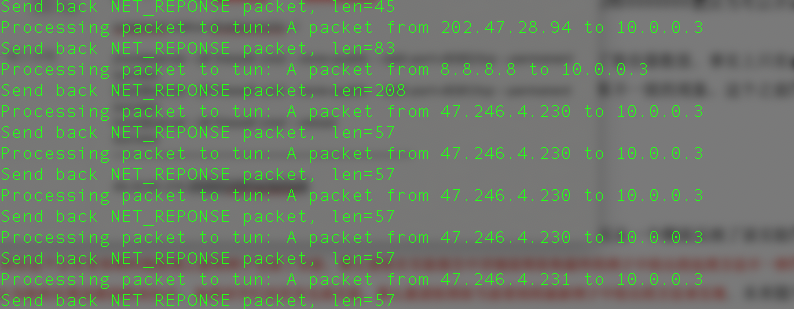
\includegraphics[scale=0.25]{./photos/2.png}%此时的图片宽度比例是相对于这个minipage的,不是全局
    \end{minipage}
    \caption{服务器运行截图}
    \label{server}
\end{figure}

\section{实验结果}
我们的安卓客户端是华为Nova,服务器运行在日本的VPS主机,提供双栈环境,使用的网络是宿舍楼的Tsinghua-5G(不进行联网认证)。我们对以下的应用进行了测试:
\begin{itemize}
    \item 通讯工具:我们对微信和QQ进行了测试,发现能够正常接收消息
    \item 视频应用:我们测试了抖音、bilibili网站。在服务器环境稳定的情况下,这些应用能够流畅的运行。
    \item 网页:我们测试了百度、bing、google等网站,能够流畅加载。
\end{itemize}
具体的运行情况还可以查看我们提供的运行效果视频。

\section{实验中遇到的问题}
我认为我们遇到的主要问题是有时候接收到错误的消息。这种情况出现的概率并不高,一般只有程序运行足够长时间后才会出现。经过我们的仔细分析,发现是由于不同线程对socket读写造成的,会造成数据错乱,因为socket的读写操作并不是原子性的。对此,网上给出的建议是将所有的写操作都统一由一个线程完成,或者使用加锁的方式。但是经过我们调研,业界对于多线程IO一个socket的做法是不推荐的,对于tcp连接来说,这样会严重影响数据传输的效率。我们实验结果显示,加锁之后,网络带宽有所降低,但是之前遇到的问题没有再次发生。这个问题一个比较好的解决思路是设置两个socket连接,单独收发,分别设立缓冲区和分隔符,使得收发数据的操作被单独封装起来,一同处理,避免出现线程安全问题。但是由于时间原因,我们没有实现。

在我们参考的相关资料中,大家并没有关注这个问题带来的隐患,如果不做处理,短时间测试不会出现问题的概率很小,但我们通过长达几十分钟乃至几小时小时的视频放映测试中发现了这个问题。

\section{实验总结}
\subsection{实验心得}
这次实验是对上学期所学的网络原理知识的综合运用。总体来说,实验的完成还是十分顺利的。通过这个实验,感觉自己对于网络方面的编程水平有了进一步的提高。看到自己编写的程序能够真正流畅运行,成就感还是相当高的。在整个实验完成的过程中,我们学习了安卓VPN service框架,掌握了epoll模型的运用,提升了服务器的性能。

再次还要感谢老师和助教的指导,没有你们,我们无法这么顺利的完成实验。

\subsection{意见和建议}
建议可以在服务器中新增一些实用路由器的一些功能,比如数据加密传输等等,提高这个实验的实用性。还有上一部分提到的多线程IO socket问题。

\end{document}
